\section{Experiments and Results}\label{sec:experiments}
\subsection{Setup}
We installed one node in each of 14 meeting rooms, with capacities from four to twelve people, for twelve weeks. Ground truth came from a ceiling-mounted counter that was installed for the study and removed afterwards. Data from ten rooms was used for training and validation; the remaining four rooms were held out for testing, so that every reported number is for rooms the model had not seen.

\subsection{Accuracy}
Table~\ref{tab:results} compares our model with two baselines: a PIR detector with a 15-minute timeout, and a gradient-boosted classifier over hand-built features that runs on a server. The quantized network loses 0.9 percentage points of detection accuracy against its floating-point version and remains well ahead of both baselines. Fig.~\ref{fig:accuracy} shows validation accuracy during training.

\begin{table}[t]
  \caption{Results on the Four Held-Out Rooms}
  \label{tab:results}
  \centering
  \begin{tabular}{lccc}
    \toprule
    Method & Detection & Count $\pm 1$ & Power \\
           & (\%)      & (\%)          & (mW) \\
    \midrule
    PIR with timeout       & 83.3 & --   & 0.12 \\
    Boosted trees (server) & 90.6 & 79.4 & 4.80 \\
    Ours, floating point   & 95.1 & 88.9 & 0.74 \\
    Ours, 8-bit            & \textbf{94.2} & \textbf{87.6} & \textbf{0.31} \\
    \bottomrule
  \end{tabular}
\end{table}

\begin{figure}[t]
  \centering
  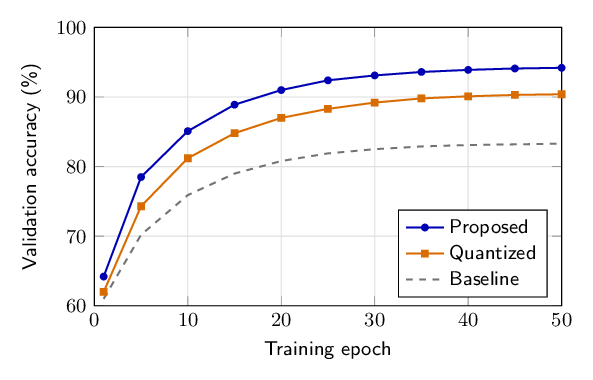
\includegraphics[width=\linewidth]{figures/accuracy.png}
  \caption{Validation accuracy during training. Quantization-aware training recovers most of the accuracy lost to 8-bit rounding.}
  \label{fig:accuracy}
\end{figure}

\subsection{Power and Energy Savings}
The node draws 0.31~mW on average, of which the radio accounts for 41\%. Two AA cells last an estimated 3.4~years. Over the final four weeks we let the estimates control the ventilation rate in seven rooms and kept the schedule in the other seven. Fan energy in the controlled rooms was 23\% lower, and carbon dioxide stayed below 1000~ppm for 99.1\% of occupied time, against 99.4\% under the schedule.

\subsection{Limitations}
All rooms are in one building with one ventilation system, and the study covered spring and early summer only. The count saturates at four or more people, which is enough for ventilation control but not for space-use planning.
